% !TEX root = mythesis.tex

%==============================================================================
\chapter{Theoretical Overview}
\label{sec:theory}
%==============================================================================

\section{Excitons}

% WAIT FOR TOM TO SEND PAPERS

% Terminology
An exciton is a bound state of electron and hole. This neutral quasi-particle is bosoniclike, meaning that it can occupy the same excitonic ground state. These composite particles are theorized to be formed when the binding energy of the electron-hole pair is bigger than the band gap. This results in an unstable ground state against spontaneous exciton generation (Fig. \ref{fig:exciton_gap}). It is worth noting that the ground state instability is important because the so called excitonic insulator is a candidate for observing a Bose-Einstein condensation transition [GROSS-NEVEU]. The excitons remind of the Cooper pairs (bound state of spin-up and spin-down electrons) used in describing superconductivity. Similarly, they form below a critical temperature and impose a quasi-particle gap [CARBON NANO TUBES]. Unlike the Cooper pairs, they do not transport charge or mass but only energy [GROSS-NEVEU]. 
% put a Graphic here
\begin{figure}[htbp]
    \centerline{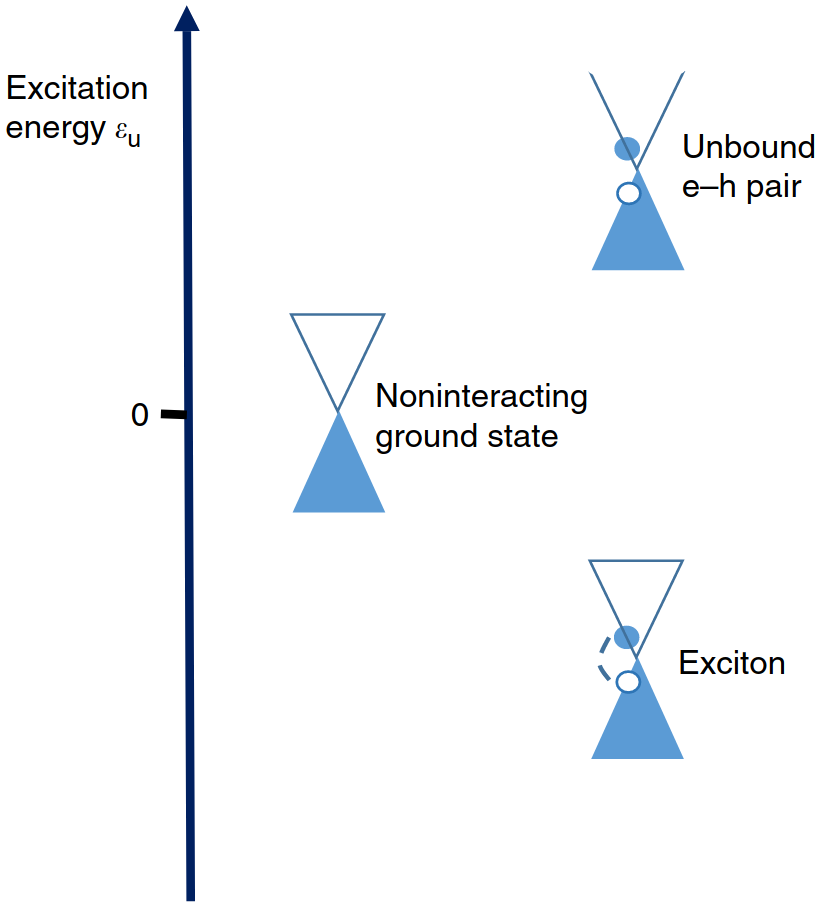
\includegraphics[width=0.35\linewidth]{exciton_gap.png}}
    % \centerline{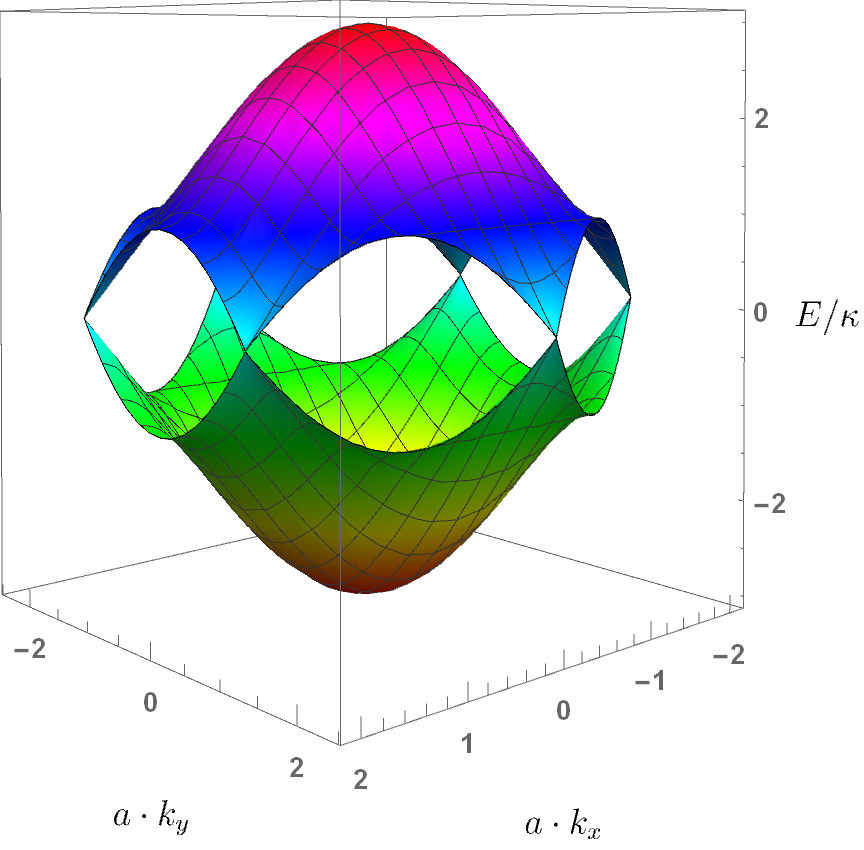
\includegraphics[width=0.7\linewidth]{band_structure.png}}
    \caption{Excitonic instability in carbon nanotubes. The scheme represents the excitation energy $\epsilon_u$ of an electron-hole (e-h) pair relative to the noninteracting ground state, a zero-gap semiconductor. In the absence of interaction, the excitation energy $\epsilon_u$ of an e-h pair is positive. The long-range interaction may bind e-h pairs close to the Dirac point in the momentum space. If an exciton forms, then its excitation energy $\epsilon_u$ is negative. This instability leads to the reconstruction of the ground state into an excitonic insulator. [CARBON NANO TUBES (took the caption word-for-word)]}
    \label{fig:exciton_gap}
\end{figure}

% Developments
In recent years, there has been a renewed interest in investigating excitons due to their theoretically proposed applications in technology. These excitonic bound states are considered to be good candidates for the development of topologically protected qubits, switching devices, and in heat exchangers [THIN-FILM TOPOLOGICAL INSULATORS(conclusion)]. The properties of the exciton have been studied on a microscopic level by employing Hubbard-like Hamiltonians on graphene lattices as well as the 3D thin-films topological insulators. There are other models (e.g. Gross-Neveu models) that have been used to describe excitons in semimetals and in semiconductors by studying the phase transitions between them and excitonic insulator. It has been shown that the dynamics of the bound electron-hole pair can be controlled in van der Waals heterostructures via a change of twist angle between the monolayers. These properties (most importantly the lifetimes of the excitons) can be tuned from the appearance of moiré potential, which in momentum space translates to relative rotation of both layer's Brillouin zones [TWIST ANGLE HETEROSTRUCTURES].
% Simulations
% On the lattice?
% Different models for excitons

In this work, we apply the Hubbard model onto a hexagonal lattice which is a model of graphene (see Section LATTICE). We are looking for the appearance of an electron-hole bound state. This will be done by measuring the binding energy of the correlation functions ratio
\begin{equation}
    \epsilon = (E_e + E_h) - E_{e-h} = \ln\left( \frac{C_e(\tau)C_h(\tau)}{C_{e-h}(\tau)} \right)
\end{equation}
The Hubbard model that we are applying there is not a mechanism for decay of the exciton state. This means that if the energy is negative ($\epsilon < 0$), we have a bound exciton state; and if the energy is higher than the energy threshold, then the particles are unbound. The study of a monolayer graphene sheets that we do in this thesis is a first step in the direction of future investigation of more complex graphene (and other) structures.


\section{The Hubbard Model}